\section{Heat Emissions}\label{heat-emissions}

Heat emissions from buildings are a crucial component influencing climate change and urban microclimate, e.g., urban heat island effect. The heat emissions from a building include heat releases from three levels of building systems: building envelope, zone/space, and HVAC systems. Quantifying heat emissions from buildings and its spatiotemporal distribution have significant implications on urban environment and climate studies. Knowing how much heat is released into the atmosphere can help quantify the magnitude of its impact on urban microclimate, e.g., urban heat island effect and climate change. Spatial and temporal distribution of heat emissions can serve to locate hot spots in space and time, therefore useful for prioritizing recourse to mitigate heat emissions from buildings.

This routine calculates heat emissions from buildings and the scope is restricted to report the buildings’ heat directly discharged to the ambient air. As shown in the figure, the emissions include heat releases from three levels of building components: (1) building envelope - exterior surface convection and radiative heat transfer to the ambient air, (2) zone - exhaust air or exfiltration to ambient, (3) HVAC system - relief/exhaust air from AHUs, and (4) HVAC system - heat rejected by air-cooled condensers or central plants, including cooling towers of water-cooled chillers, gas-fired boilers, furnaces and water heaters. It should be noted that any under-ground zone or envelope is excluded, since heat from those spaces is rejected to ground instead of to ambient air. 

\begin{figure}[hbtp] 
\centering
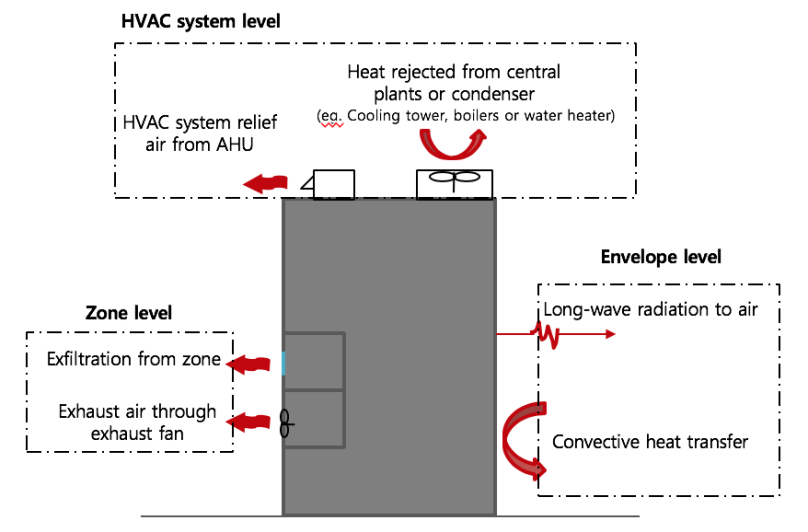
\includegraphics[width=0.9\textwidth, height=0.9\textheight, keepaspectratio=true]{media/heatemission.png}
\caption{Building released heat compositions \protect \label{fig:building-released-heat-compositions}}
\end{figure}

The calculated heat emissions measure the heat transfer from buildings to their ambient environment, and can have both positive and negative values. The positive values indicate the building injects heat to the environment, while the negative values indicate the building extracts heat from the environment.

For heat transfer via air flow, both the sensible and latent heat emissions are calculated and reported.

\subsection{Heat Emission from Building Envelope}\label{emission-from-envelope}

Exterior surfaces emit heat to ambient air in the form of convection and long-wave radiation, which could be absorbed by particles and gas molecules in air. The internal sources modify the outside surface temperature through envelope conduction, along with incident solar radiation, which triggers the heat exchange with the ambient air. This part does not include the long-wave radiation from surfaces to the sky or the ground. The surface outside face heat emission rate is calculated as:

\begin{equation}  \label{eq:he-1}
Q_{emission, surf} = Q_{conv, surf} +  Hr * A * (T_{surf} - T_{out})
\end{equation}

where \(Q_{conv, surf}\) is the surface outside face convection heat gain rate, \(Hr\) is the surface outside face thermal radiation to air heat transfer coefficient, \(A\) is the surface area, \(T_{surf}\) and \(T_{out}\) are the surface and outdoor air temperature.

\subsection{Heat Emission from Zones}\label{emission-from-zones}

Discharge air carries heat to ambient at the zone level from exfiltration and exhaust fan. Exfiltration is unintended airflow to outside through envelope cracks, as opposite to infiltration. Zones such as restroom, kitchen and laundry room may be equipped with exhaust fans for active venting. These items can be quantified by:

\begin{equation}  \label{eq:he-2}
Q_{exf, zone} = m_{exf}(h_{zone} - h_{out})
\end{equation}

\begin{equation}  \label{eq:he-3}
Q_{exh, zone} = m_{exh}(h_{zone} - h_{out})
\end{equation}

where \(m_{exf}\) is the exfiltration air mass flow rate, \(m_{exh}\) is the zone exhaust air mass flow rate from the zone exhaust node, \(h_{zone}\) and \(h_{out}\) are the zone and outdoor air enthalpy. Among these, the sensible parts are:

\begin{equation}  \label{eq:he-4}
Q_{exf, zone, sensible} = m_{exf} * c * (T_{zone} - T_{out})
\end{equation}

\begin{equation}  \label{eq:he-5}
Q_{exh, zone, sensible} = m_{exh} * c * (T_{zone} - T_{out})
\end{equation}

where \(c\) is the specific heat of air, \(T_{zone}\) and \(T_{out}\) are the zone and outdoor air temperature. And the latent parts are determined by taking the difference between the total and the sensible rate. For each zone, its exfiltration rate is calculated by solving a mass flow balance on the zone including infiltration, ventilation, outdoor air mixing, zone-to-zone mixing, and all of the zone inlet, exhaust, and return nodes.

This part of zone exhaust only includes the exhaust heat at the zone level defined by \textbf{Fan:ZoneExhaust} or \textbf{AirflowNetwork:MultiZone:Component:ZoneExhaustFan}. For each zone, we aggregated this part by searching its exhaust fans. The exhaust heat from Zone HVAC system nodes is included in the next item.

\subsection{Heat Emission from HVAC Systems through Relief Air}\label{emission-from-HVAC-relief}

HVAC systems relieve heat from system outdoor air relief nodes, and the total and sensible emission rate are calculated as:

\begin{equation}  \label{eq:he-6}
Q_{exh, sys} = m_{exh}(h_{node} - h_{out})
\end{equation}

\begin{equation}  \label{eq:he-7}
Q_{exh, sys, sensible} = m_{exh} * c * (T_{node} - T_{out})
\end{equation}

And the latent parts are determined by taking the difference between the total and sensible rate.

The air exchange with outdoor is represented with an \textbf{OutdoorAir:Mixer} object in the \textbf{AirLoopHVAC:OutdoorAirSystem} object. This part is aggregated and reported by each \textbf{Controller:OutdoorAir} object.

\subsection{Heat Rejection from HVAC System Equipment}\label{emission-from-HVAC-reject}

HVAC system equipment also directly exchanges heat with ambient air via refrigeration cycle and its energy usage. For example, for gas-fired boilers/heaters, waste heat is exhausted to outside together with combustion byproduct. For space cooling, heat is removed from indoors and dumped to outdoor at the condenser side or corresponding cooling equipment, such as cooling tower. In addition, energy consumed by outdoor equipment will directly dissipate to the ambient air, such as compressors and fans in packaged DX systems. The surface outside face heat emission rate is calculated as:

(1)	Gas-powered combustion unit: Fuel generated heat - fuel heat supply

(2)	Condensing unit:

a.	Air-cooled: cooling rate + electric power of condenser fan and compressor

b.	Water-cooled: total heat transfer rate with outdoor air

Detailed calculation of HVAC rejected heat varies with different HVAC object groups and component types, as summarized in Table~\ref{table:emission-from-hvac-components}.

% table 94
\begin{longtable}[c]{p{1.0in}p{2.0in}p{3in}}
\caption{Heat Rejection Calculation for Different HVAC Component Types \label{table:emission-from-hvac-components}} \tabularnewline
\toprule 
Object Group & Component & Calculation Methods \tabularnewline
\midrule
\endhead
Coils      & Chilled water cooling coil   & Emit heat in condensing unit defined in Condenser Equipment \tabularnewline
           & Heating coil (fuel heated)   & Fuel Consumed + Heating Coil Defrost Electric Consumption + Heating Coil Crankcase Heater Electric Consumption – Heating Coil Total Heating Energy \tabularnewline
           & Hot water/steam heating coil & Emit heat in plant source defined in Plant Heating and Cooling Equipment \tabularnewline
           & DX cooling coil (air-cooled) & Cooling Coil Source Side Heat Transfer Rate + Cooling Coil Electric Power + Cooling Coil Crankcase Heater Electric Energy + Fuel Waste Heat \tabularnewline
           & DX cooling coil (Evaporatively-cooled)  & Evaporative Cooler Condenser Pump Electricity Consumption + Cooling Coil Basin Heater Electric Energy + Evaporative Cooler Water Volume * rho * evaporation heat of water (\(\delta H_{we}\)) \tabularnewline
           & DX VRF cooling coil          & Emit heat in condensing unit defined in Variable Refrigerant Flow Equipment \tabularnewline
           & DX heating coil (air-cooled) & Heating Coil Electric Power / Fuel Consumed + Heating Coil Defrost Electric Power + Heating Coil Crankcase Heater Electric Power – Heating Coil Total Heating Rate \tabularnewline
           & Water to air heat pump       & Emit heat in condensing unit defined in Condenser Equipment \tabularnewline
           & DX VRF cooling /heating coil & Emit heat in condensing unit defined in Variable Refrigerant Flow Equipment \tabularnewline

Evaporative Coolers                 & Evaporative Coolers & Evaporative Cooler Condenser Pump Electricity Consumption + Cooling Coil Basin Heater Electric Energy + Evaporative Cooler Water Volume * rho * evaporation heat of water (\(\delta H_{we}\)) \tabularnewline
Variable Refrigerant Flow Equipment & VRF air-to-air heat pump condensing unit (air-cooled) & VRF Heat Pump Total Cooling Rate + VRF Heat Pump Total Electric Power (cooling mode)<br>VRF Heat Pump Total Heating Electric Power / Fuel Rate - VRF Heat Pump Total Heating Rate (heating mode) \tabularnewline
                                    & VRF air-to-air heat pump condensing unit (evaporative-cooled) & Evaporative Cooler Condenser Pump Electricity Consumption + Cooling Coil Basin Heater Electric Energy + Evaporative Cooler Water Volume * rho * evaporation heat of water (\(\delta H_{we}\)) \tabularnewline
                                    & VRF air-to-air heat pump condensing unit (water-cooled) & VRF Heat Pump Condenser Heat Transfer Rate \tabularnewline
Plant Heating and Cooling Equipment & Hot water/Steam boiler & Boiler <Fuel Type> Rate + Boiler Ancillary Electric Energy - Boiler Heating Rate \tabularnewline
                                    & Chiller water-cooled & Emit heat in Condenser Equipment \tabularnewline
                                    & Chiller air-cooled / evap-cooled & Chiller Condenser Heat Transfer Rate \tabularnewline
Condenser Equipment                 & Cooling Tower & Cooling Tower Heat Transfer Rate + Cooling Tower Fan Electric Power \tabularnewline
Water Heaters and Thermal Storage   & Water heater & Water Heater <Fuel Type> Rate - Water Heater Heating Rate \tabularnewline
Zone HVAC Forced Air Units          & Window air conditioner / Packaged terminal air conditioner (PTAC) / Packaged terminal heat pump (PTHP); Energy recovery ventilator (ERV); Unit ventilator/heater; Zone outdoor air unit & <unit type> Total Cooling Rate + <unit type> Electric Energy (cooling mode)<br><unit type> Heating Electric Power / Fuel Rate + <unit type> Electric Power - <unit type> Total Heating Rate (heating mode) \tabularnewline
                                    & Water-to-air heat pump & Emit heat in condensing unit defined in Condenser Equipment \tabularnewline
                                    & Zone evaporative cooler & Emit heat in condensing unit defined in Evaporative Coolers \tabularnewline
                                    & Hybrid Unitary HVAC & System dependent; Calculated according to the equipment specification as above \tabularnewline
\bottomrule
\end{longtable}

There are several types of components for which the heat rejection is not clearly defined. The following are not included in the heat emissions report:

\begin{itemize}
  \item User defined systems have a variety of possible sources of heat emission including outdoor air relief for exhaust or a condenser outlet for heat rejection. These parts can be counted by tracing the condensing unit linked to the air connection inlet and outlet (for user defined zone HVAC and plant component). 
  \item For user defined coil, this part depends on how the coil is designed and equipped. We do not count this in report.
  \item ThermalStorage:Ice:* do not indicate where losses go, so we neglect this.
\end{itemize}

By summing up these components, the heat emissions are calculated and reported from buildings by systems and components as well as in total.
